\section{Method}
We started the study with a setup of sampling calorimeter consisting of alternating lead sheet and strips of the plastic scintillator as shown in Fig.~\ref{fig:det_conf}. The electromagnetic shower mainly generated at the lead sheet (passive component) due to its short radiation length ($X_0 = 5.6~{\rm mm})$ and the information of the shower particles is obtained by using the scintillator (active  component). The thickness of lead is 1 mm and scintillator is 5 mm, respectively. The lead sheet has a cross-section of  500 mm $\times$ 500 mm and the scintillator strip of 500 mm $\times$ 15 mm. By arranging the strips in X- and Y-direction alternatively along Z-direction. The generated photon moves along with Z-direction and its incident angle was defined as a polar angle to the direction.  With the configuration, we can get shower profiles in X- and Y-axis in turn, and estimate the incident angle from them. The number of alternating layers is 105, corresponding to 20 radiation length (Xo), in order to contain shower particles fully. 

\begin{figure}[!hbt]
%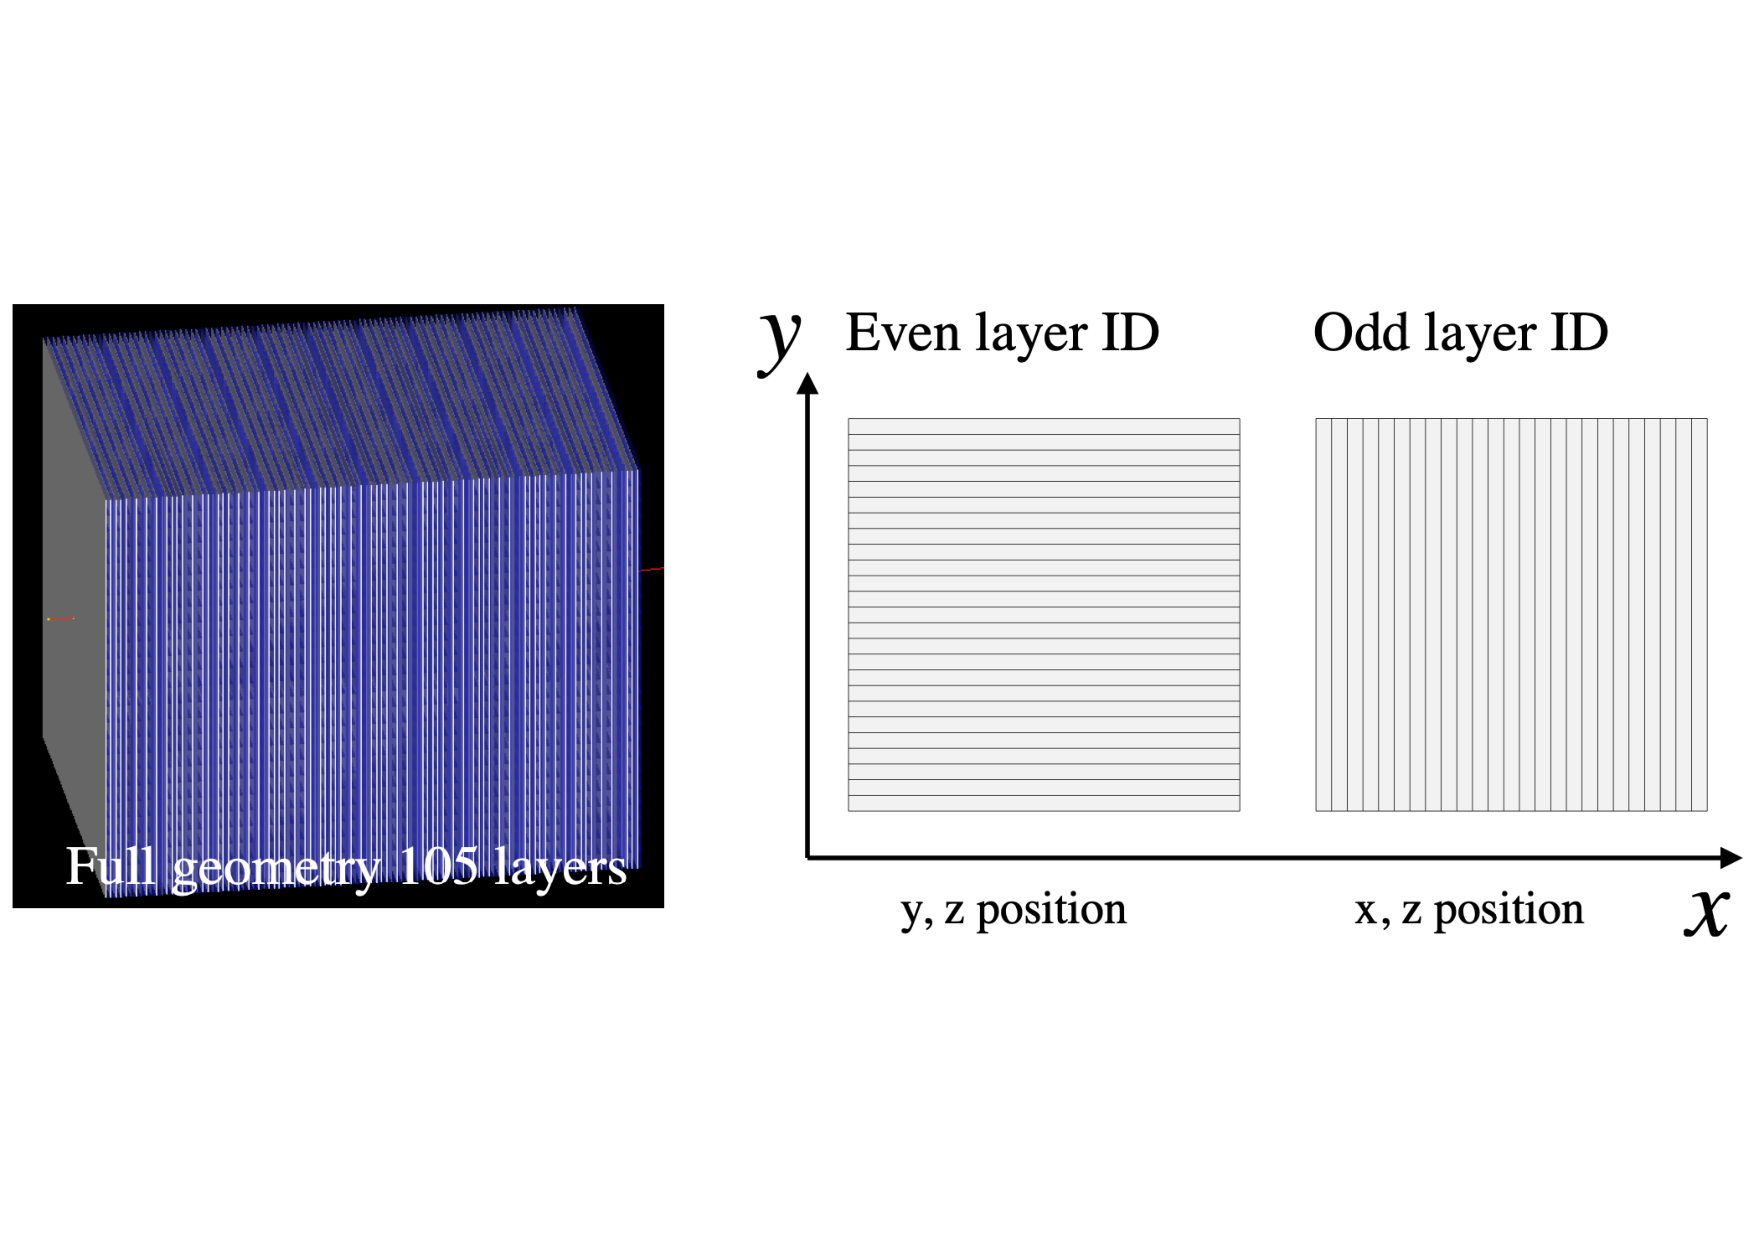
\includegraphics[width=0.85\textwidth]{figures/Sec2/ang_conf.pdf}
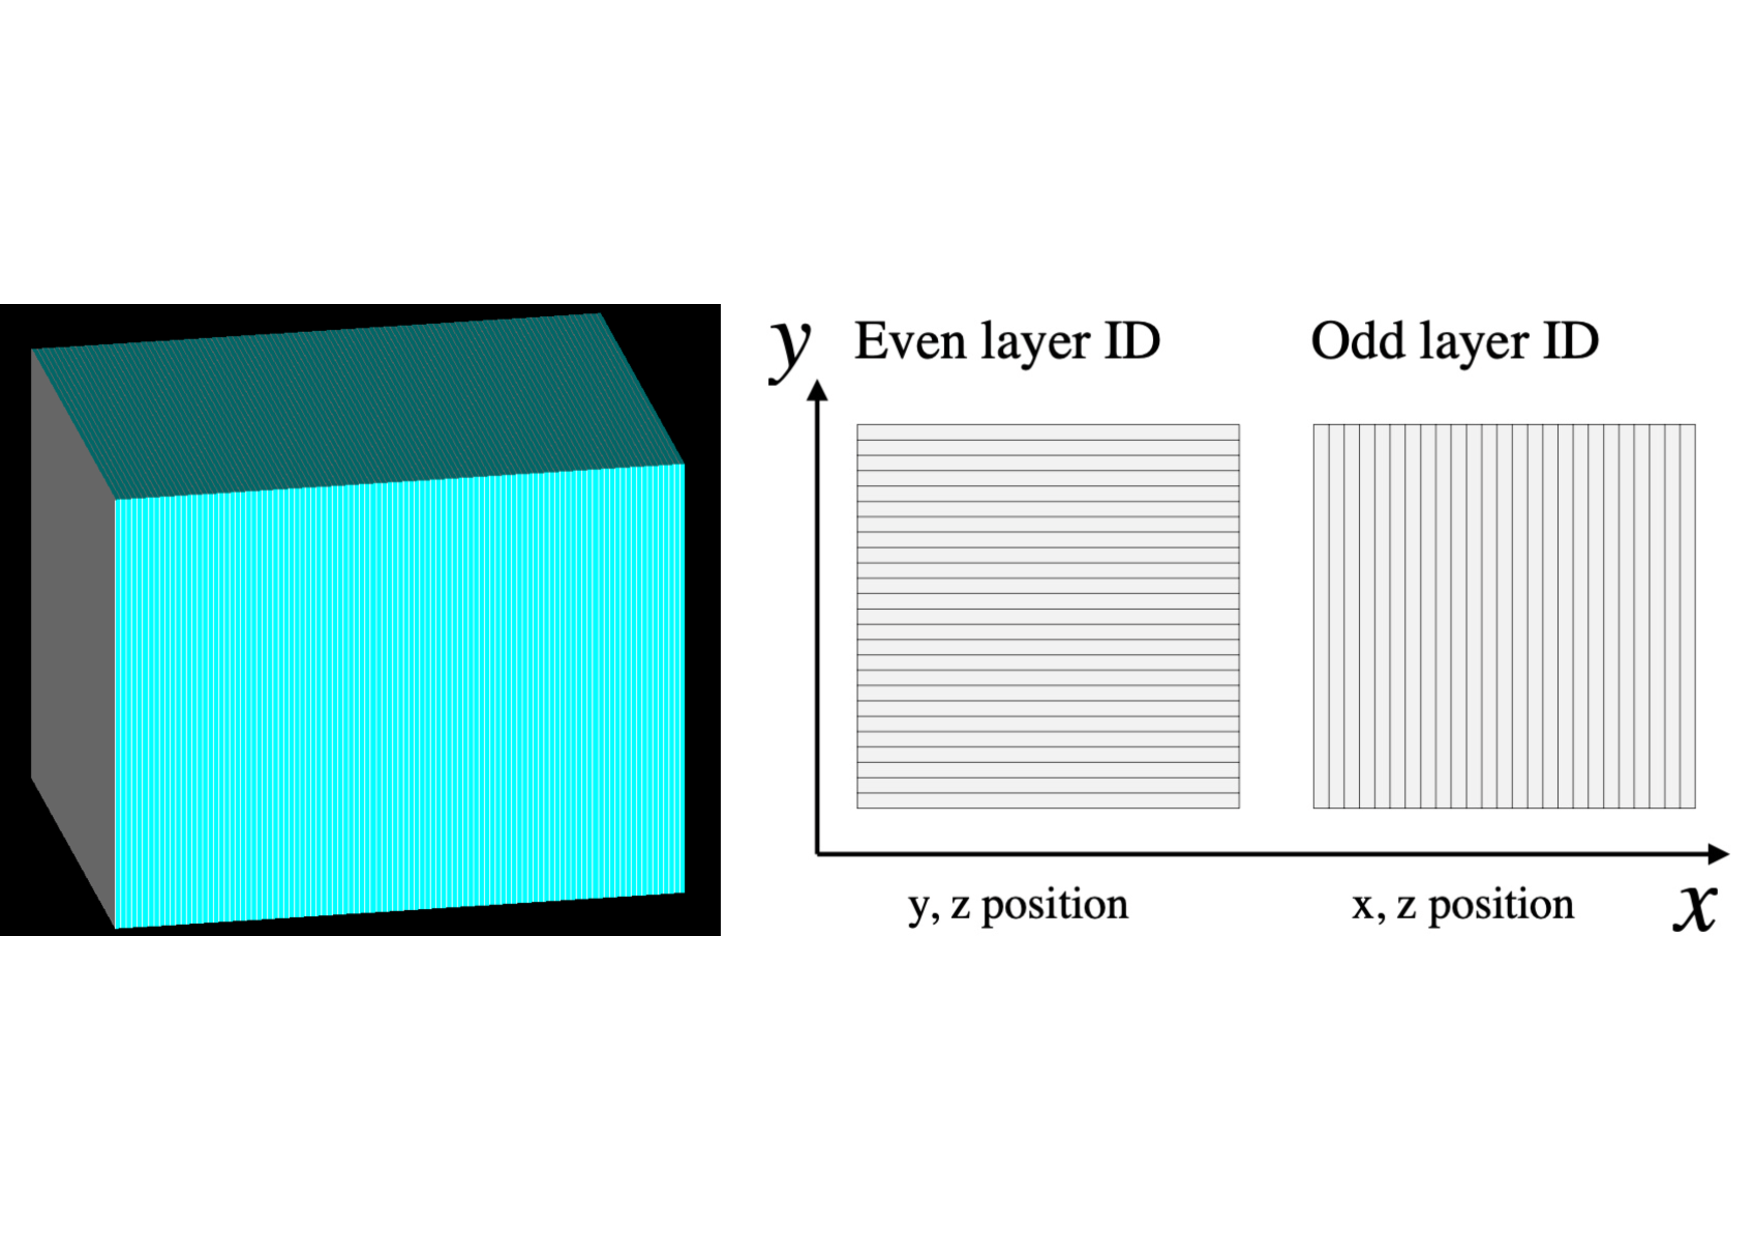
\includegraphics[width=0.85\textwidth]{figures/Sec2/Prototype_samplingcal.pdf}

\caption{ The first trial of detector setup for simulation study on angle measurement. It is a sampling calorimeter consisting of alternating lead sheets and strips of plastic scintillator. }
\label{fig:det_conf}
\end{figure}

The electromagnetic showers are generated with given detector setup by using the GEANT4 package (ver. xxx) with the standard EM sub-packages (URL: https://geant4.web.cern.ch/node/1828). 
${\it I will describe the coordinator}$
%The contribution of the hadronic interaction is taken into account with $\rm{FTFP\_BERT}$ package. The materials used in detector construction are selected from the Geant4 NIST material database: $\rm{G4\_Pb}$ for the lead and $\rm{G4\_PLASTIC\_SC\_VINYLTOLUENE}$ for the scintillator material.

In order to reconstruct the incident angle of the gamma, we used the $\XGB$, which is one of the machine learning packages supporting a scalable tree boosting system~\cite{xgboost:2016}. Input data for the $\XGB$ are deposit energies on each scintillator strip by the generated shower particles. It includes the strips of zero-energy deposit in order to satisfy the requirement that the number of input data should be identical. As the training procedure, the $\XGB$ studies profiles of energy deposit to the individual strips with respect to the incident angle for a given $\gamma$ energy. 

There are five hyperparameters which can be set by user, and their values are selected to provide the better angular resolution as described in tab.~\ref{tab:XgbPar}. Among these hyperparameters, the Max. depth rapidly improves the angular resolution with increasing its value until 100. The N\_estimators also improves the angular resolution with increasing its number up to 1,000 and N\_estimators larger than 1000 does not change the resolution. Its optimal condition becomes 1000 with the Max. depth is 100.

\begin{table}[hbt!]
\centering
\caption{Parameterization of the $\XGB$}
\begin{tabular}{cccc}
\hline 
Parameter & Function & Default value & Used value \\ \hline 
N\_estimators & The number of decision trees & N.A. & 1000 \\  
Max. depth & Possible maximum depth of tree structure & 6 & 100 \\ 
Subsample & Fraction of total data used for a single decision & 1 & 1 \\ 
Learning rate & Step length for calculation & 0.3 & 0.08 \\ 
Gamma & Requirement on minimum loss function & 0 & 0 \\ 
\hline
\end{tabular}
\label{tab:XgbPar}
\end{table}

For the training procedure, gammas are generated uniformly in the range 0 to 50 degrees of polar angle ($\theta$) and  0 to 360 degrees of azimuthal angle ($\varphi$). The performance of the angular reconstruction is tested with independently generated data samples with fixed $\theta$ and uniform $\varphi$ from 0 to 360 degrees.

